\documentclass[14pt,a4paper]{extarticle}
\usepackage{../templates/preamble}

\newcommand{\reportof}{практической работе №3}
\newcommand{\theme}{Аппроксимация и преобразования функций.}

\begin{document}
\begin{titlepage}
    \begin{center}
        {\bfseries
        МИНОБРНАУКИ РОССИИ\par
        САНКТ-ПЕТЕРБУРГСКИЙ ГОСУДАРСТВЕННЫЙ\par
        ЭЛЕКТРОТЕХНИЧЕСКИЙ УНИВЕРСИТЕТ\par
        <<ЛЭТИ>> ИМ. В.И. УЛЬЯНОВА (ЛЕНИНА)\par
        Кафедра \department

        \vspace{0.23\textheight}
        ОТЧЁТ\par
        по \reportof\par
        по дисциплине <<\discipline>>\par
        Тема: \theme
        \vspace{0.28\textheight}
        }
        \begin{table}[!ht]
            \begin{tabularx}{\textwidth}{p{60mm}X>{\centering\arraybackslash}p{45mm}}
                Студент гр. 4352 & \_\_\_\_\_\_\_\_\_\_\_\_\_\_\_\_\_\_\_\_ & {Даричев Е. М.} \\ [5.4mm]  % Line height
                Преподаватель    & \_\_\_\_\_\_\_\_\_\_\_\_\_\_\_\_\_\_\_\_ & {\teacher} \\ [5.4mm]
            \end{tabularx}
        \end{table}

        Санкт-Петербург\par
        \yyear
    \end{center}
\end{titlepage}
\setcounter{page}{2}

\section*{Цель работы}
мяу мяу


\section*{Отчёт о проделанной работе}
        Напишем для первого задания функцию, которая будет считать среднеквадратичной
ошибки и посчитаем его для заданных точек и функций (рис. \ref{fig:3.1}).

\begin{figure}[h!]
    \centering
    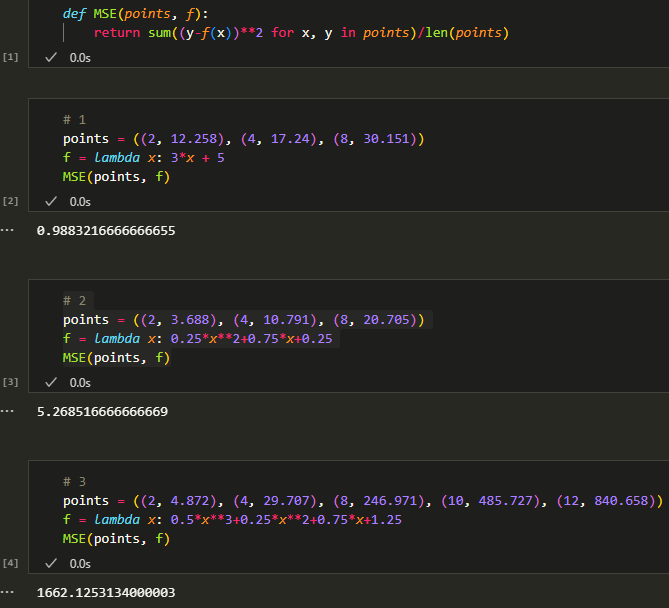
\includegraphics[width=0.7\linewidth]{figures/3.1.png}
    \caption{Нахождение среднеквадратичной ошибки}
    \label{fig:3.1}
\end{figure}

        Во втором задании необходимо подобрать функции под данные точки так, чтобы
значение MSE было меньше определенного значения. Первая функция --- линейная
($x+5$, рис. \ref{fig:3.2-start1}). Повернём прямую, изменив коэффициент перед
первой степенью переменной. При значении $-14$ MSE имеет значение $\approx 103$ (рис.  \ref{fig:3.2-1}).
Вторая функция является кубической параболой (рис. \ref{fig:3.2-start2}). Переместим
её влево, добавив ко всем значениям переменной константу. При $k=20$, $MSE=141$.
\newpage

\begin{figure}[h!]
    \begin{subfigure}{.5\textwidth}
        \centering
        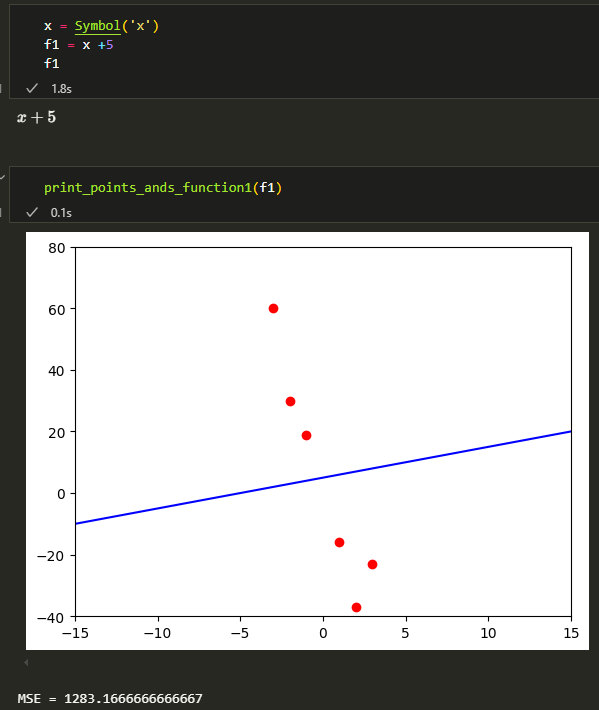
\includegraphics[width=0.9\linewidth]{figures/3.2-start1.png}
        \caption{Линейная функция}
        \label{fig:3.2-start1}
    \end{subfigure}%
    \begin{subfigure}{.5\textwidth}
        \centering
        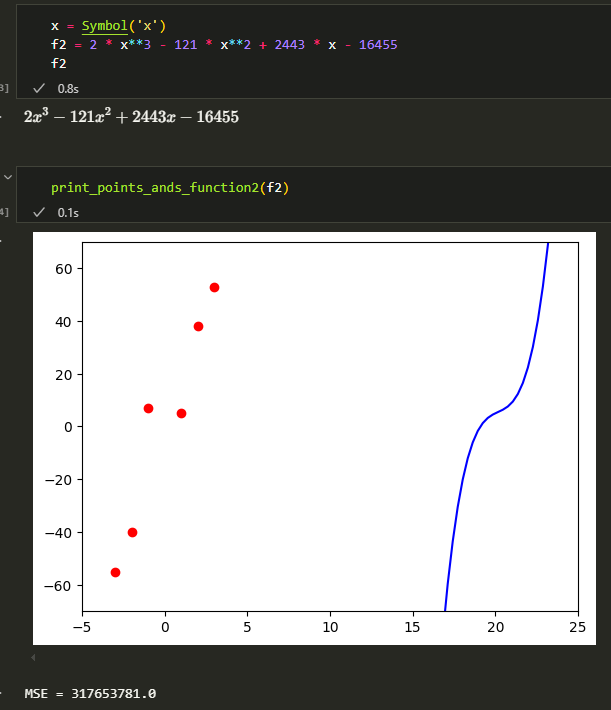
\includegraphics[width=0.9\linewidth]{figures/3.2-start2.png}
        \caption{Кубическая парабола}
        \label{fig:3.2-start2}
    \end{subfigure}

    \caption{Задание 3.2, начальные состояния}
    \label{fig:2.1-start}
\end{figure}

Ниже на рисунке \ref{fig:2.1} представлены результаты работы.

\begin{figure}[h!]
    \begin{subfigure}{.5\textwidth}
        \centering
        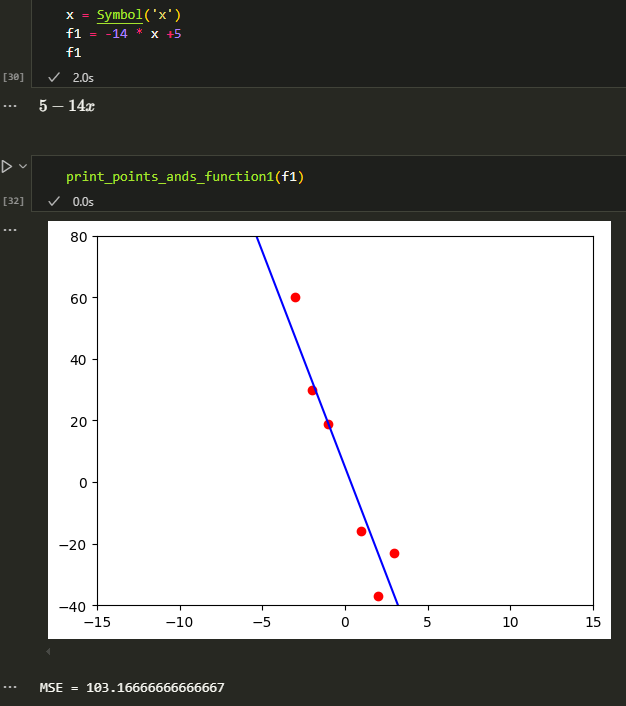
\includegraphics[width=0.9\linewidth]{figures/3.2-1.png}
        \caption{$k=-14$}
        \label{fig:3.2-1}
    \end{subfigure}%
    \begin{subfigure}{.5\textwidth}
        \centering
        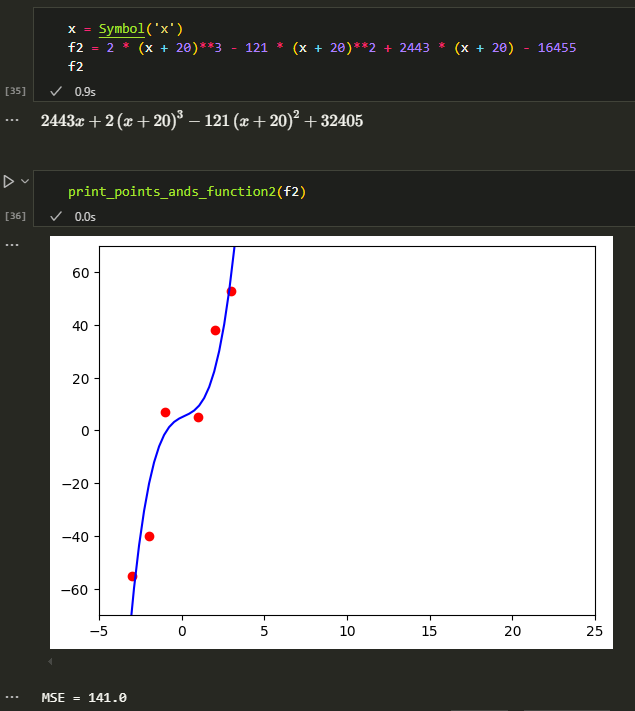
\includegraphics[width=0.9\linewidth]{figures/3.2-2.png}
        \caption{$k=-20$}
        \label{fig:3.2-2}
    \end{subfigure}

    \caption{Задание 3.2, результаты}
    \label{fig:2.1}
\end{figure}

        В следующем задании нужно получить значение среднеквадратичной
ошибки меньше 50 для функции $3.375 x ^ 3 - 9 x^2$. Разделим аргумент на $1.5$ и
прибавим к функции $4.5$ (рис. \ref{fig:3.3}). Далее для функции $0.074 x^3 - 0.11 x^2 + x + 5$
необходимо получить MSE меньше 200.

\begin{figure}[h!]
    \begin{subfigure}{.5\textwidth}
        \centering
        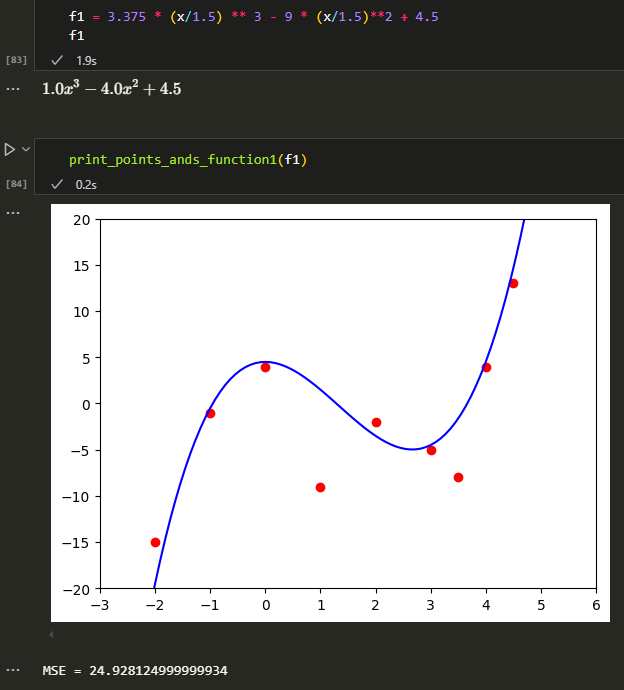
\includegraphics[width=0.95\textwidth]{figures/3.3-1.png}
        \caption{Первая часть}
        \label{fig:3.3.1}
    \end{subfigure}%
    \begin{subfigure}{.5\textwidth}
        \centering
        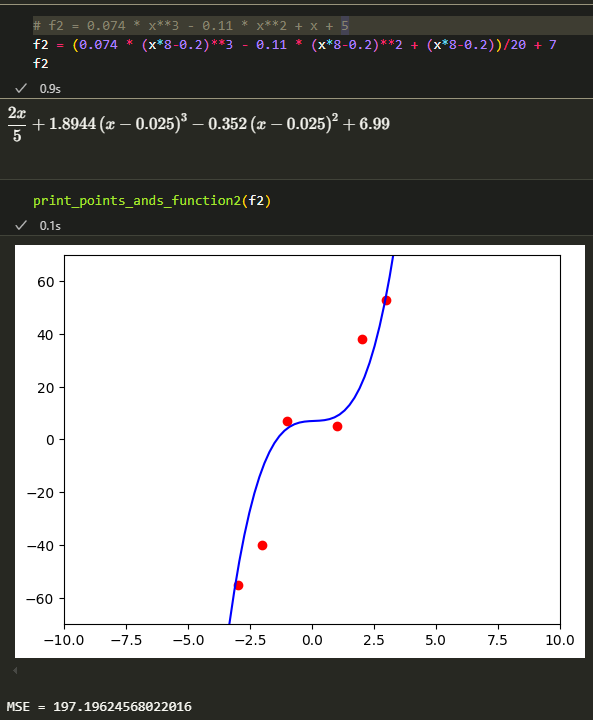
\includegraphics[width=0.95\textwidth]{figures/3.3-2.png}
        \caption{Вторая часть}
        \label{fig:3.3.2}
    \end{subfigure}
    \caption{Задание 3.3}
    \label{fig:3.3}
\end{figure}

        В первом блоке следующего задания необходимо найти полиномы,
описывающие набор точек. На рисунке \ref{fig:3.4code} представлен код
для решения этого блока, а на рисунке \ref{fig:3.4block1} --- результаты
работы.

\begin{figure}[h!]
    \centering
    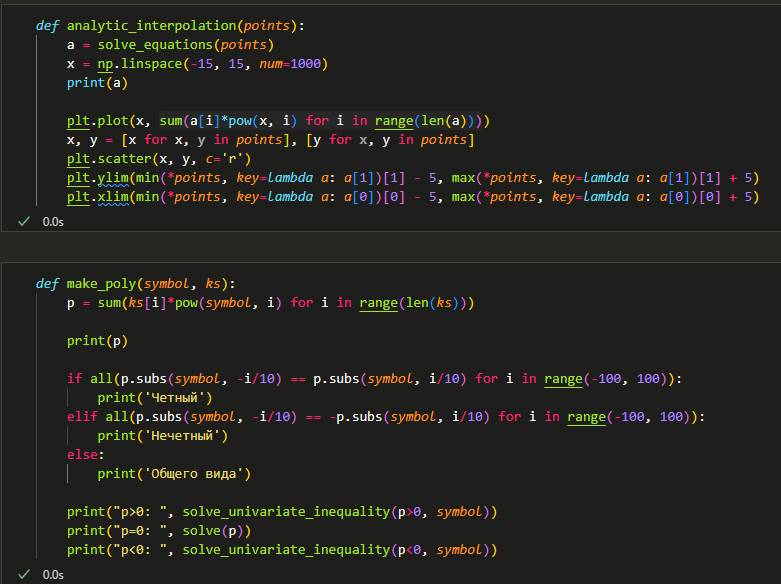
\includegraphics[width=0.65\textwidth]{figures/3.4 code.png}
    \caption{Код задания 3.4}
    \label{fig:3.4code}
\end{figure}

\begin{figure}[ht!]
    \begin{subfigure}{.5\textwidth}
        \centering
        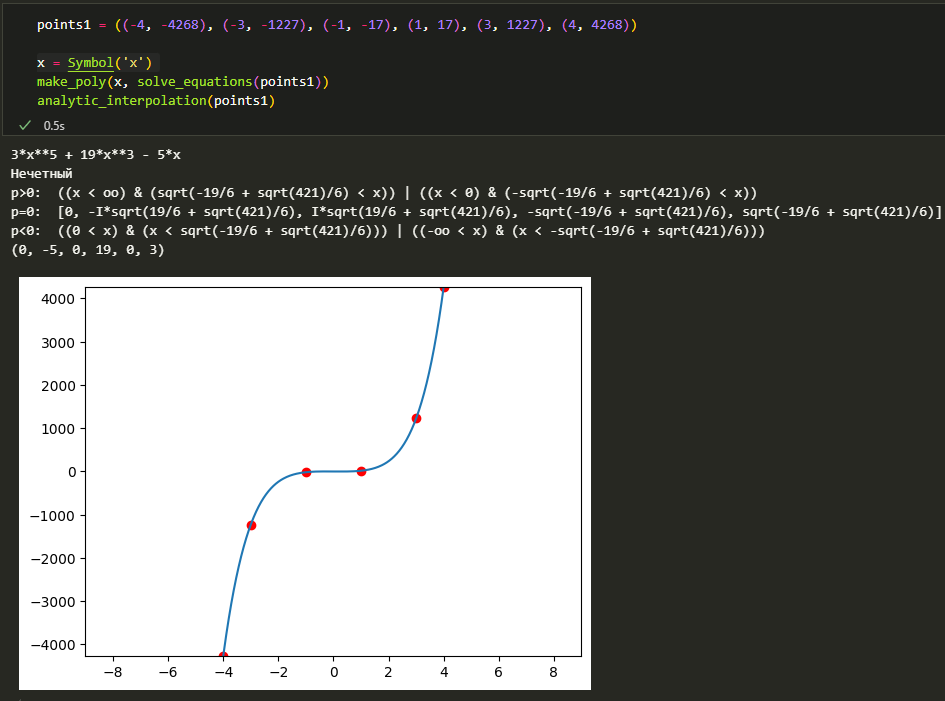
\includegraphics[width=0.95\textwidth]{figures/3.4-1-1.png}
    \end{subfigure}%
    \begin{subfigure}{.5\textwidth}
        \centering
        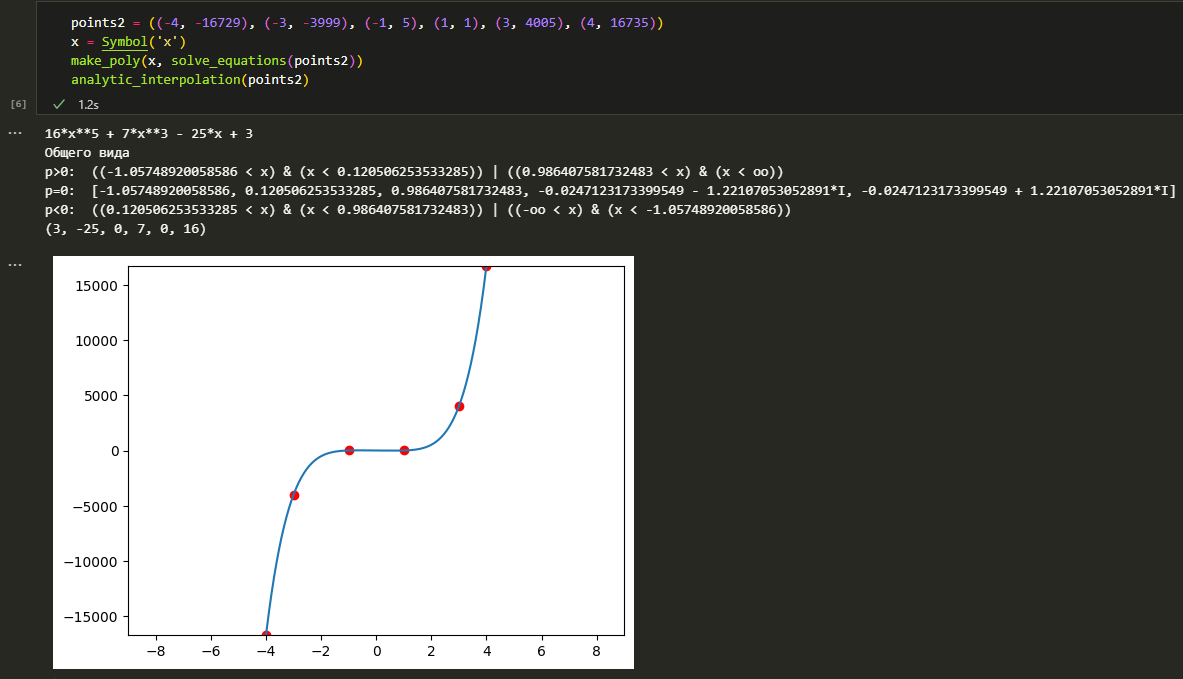
\includegraphics[width=0.95\textwidth]{figures/3.4-1-2.png}
    \end{subfigure}
    \caption{Задание 3.4}
    \label{fig:3.4block1}
\end{figure}

        Во втором блоке необходимо так же получить MSE меньше
определенного значения. Для $48x^2 - 128x + 83$ получить MSE
меньше $5$ (рис. \ref{fig:3.4-1}). Для $4x^3 + 30x^2 + 74x + 62$
получить MSE меньше $35$ (рис. \ref{fig:3.4-2}). Для $-36 x^3 - 
756 x^2 - 5334 x - 12636$ получить MSE $< 3300$ (рис. \ref{fig:3.4-3}).
Для $- \frac{5}{4} x^2 + 25x - 152$ получить MSE $<25$ (рис. \ref{fig:3.4-4}).

\begin{figure}[ht!]
    \begin{subfigure}{.5\textwidth}
        \centering
        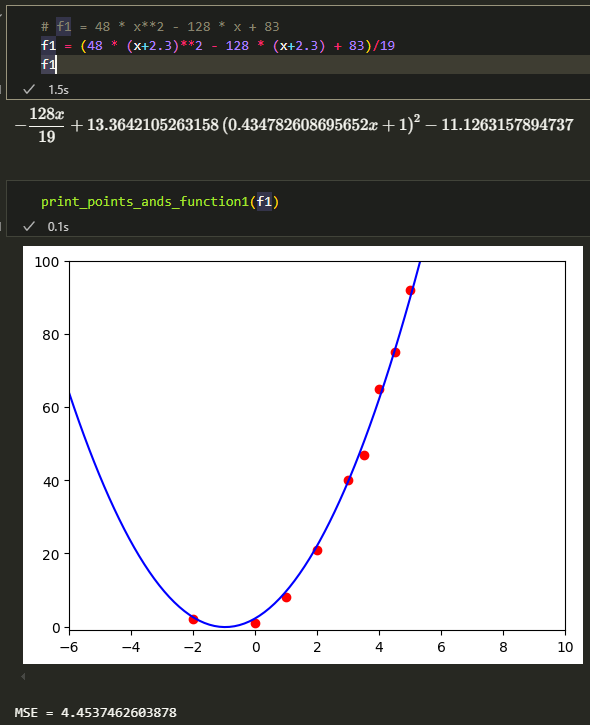
\includegraphics[width=0.95\textwidth]{figures/3.4 1.png}
        \caption{Полином №1}
        \label{fig:3.4-1}
    \end{subfigure}%
    \begin{subfigure}{.5\textwidth}
        \centering
        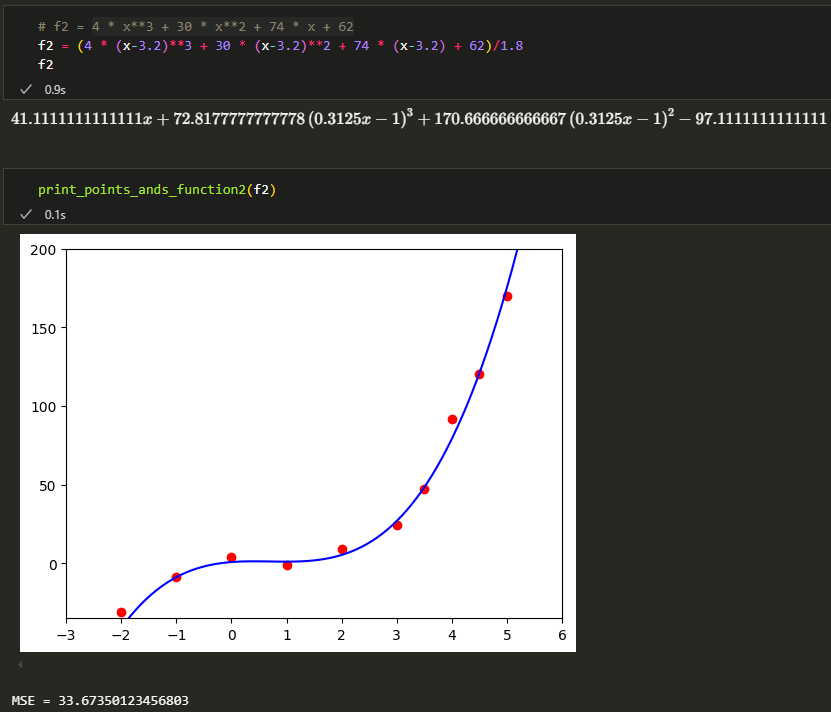
\includegraphics[width=0.95\textwidth]{figures/3.4 2.png}
        \caption{Полином №2}
        \label{fig:3.4-2}
    \end{subfigure}%
    \caption{Первая половина блока}
    \label{fig:3.4block2-1}
\end{figure}

\begin{figure}[ht!]
    \begin{subfigure}{.5\textwidth}
        \centering
        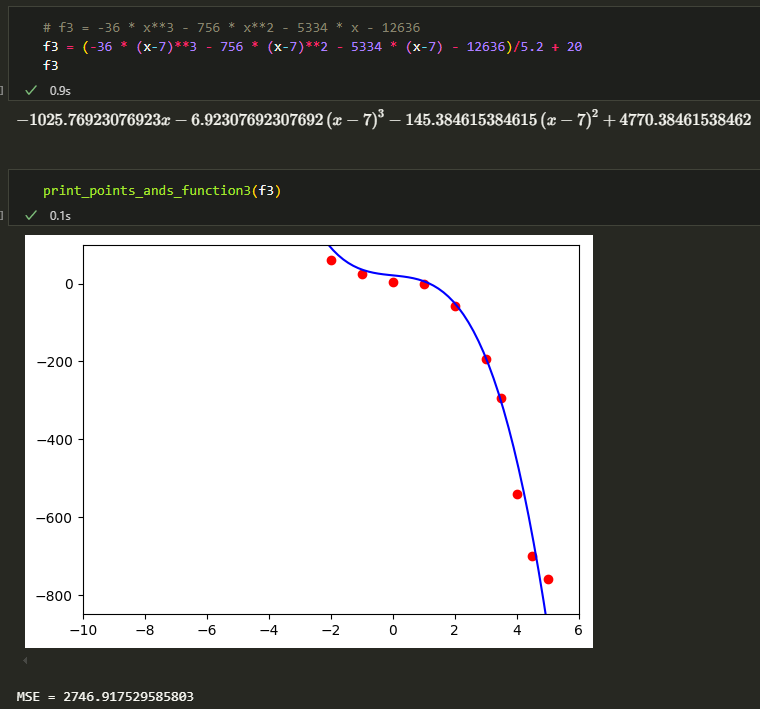
\includegraphics[width=0.95\textwidth]{figures/3.4 3.png}
        \caption{Полином №3}
        \label{fig:3.4-3}
    \end{subfigure}%
    \begin{subfigure}{.5\textwidth}
        \centering
        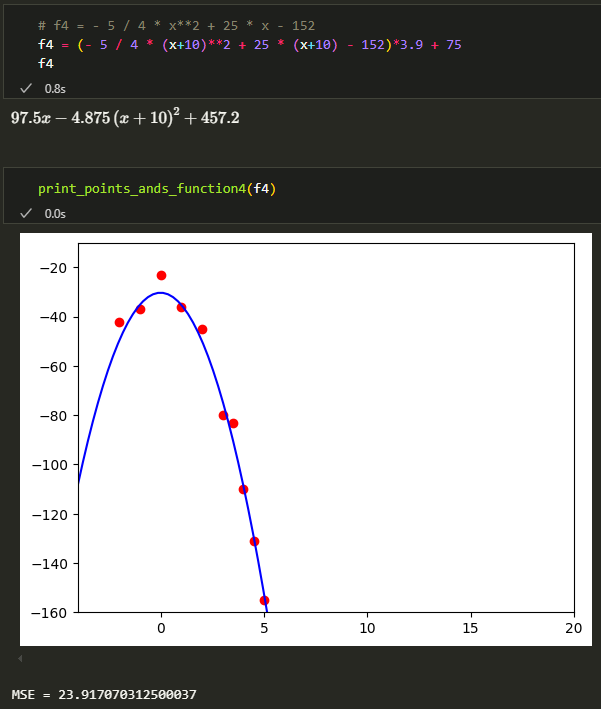
\includegraphics[width=0.95\textwidth]{figures/3.4 4.png}
        \caption{Полином №4}
        \label{fig:3.4-4}
    \end{subfigure}%
    \caption{Вторая половина блока}
    \label{fig:3.4block2-2}
\end{figure}

\section*{Вывод}

        В ходе выполнения работы я познакомился с среднеквадратичной
ошибкой, как её находить, узнал о различных преобразованиях функций.

\end{document}